% sections/17_confine1d.tex  —  Confinement demo (figure + σ table)
% Plan ref: §17  ▲ Fig 17-1  • Tbl σ values

\section{Confinement Demo in \(1+1\) D}
\label{sec:confine1d}

\paragraph{Recap.}
We discretise a unit‐length channel into \(N=256\) sites; the mobility
tensor is \(A^{xx}=D(x)\) with a low-mobility barrier in
\(\tfrac14L<x<\tfrac34L\) (Sec.~\ref{sec:info_force}).  The initial
entropy spike sits at \(x=\tfrac18L\).

\paragraph{Steady‐state density.}
The Crank–Nicolson solver in \texttt{src/lattice\_M1.py} evolves
\(\partial_t\rho = \partial_x(D\partial_x\rho)\) to steady state.
Figure~\ref{fig:entropy_density} shows the resulting confinement; 
Fig.~\ref{fig:lattice_potential} shows the sinusoidal barrier used.


% ---------- Figure 3 – potential ----------
\begin{figure}[ht]
  \centering
  \resizebox{.72\linewidth}{!}{% figs/lattice_potential.tex  – 1-D sinusoidal lattice potential
\begin{tikzpicture}[x=0.8cm, y=0.55cm, >=stealth, font=\small]
  % axes
  \draw[->] (-0.3,0) -- (6.4,0) node[below] {$x$};
  \draw[->] (0,-1.1) -- (0,1.3) node[left] {$V(x)$};

  % potential V(x)=sin x
  \draw[thick, blue!70, samples=200, smooth, domain=0:6.2]
        plot (\x,{sin(\x r)});

  % minima markers
  \foreach \k in {1,3,5}{
    \fill [red!70] (\k*pi/2,0) circle [radius=1.2pt];
  }

  % label
  \node[above right] at (4.2,-0.7) {$V_0\sin\!\bigl(\tfrac{2\pi}{a}x\bigr)$};
\end{tikzpicture}
}%
  \caption{One-dimensional sinusoidal confinement potential used in the Kick-lattice toy model. Red dots mark the minima.}
  \label{fig:lattice_potential}
\end{figure}

% ---------- Figure 4 – entropy density ----------
\begin{figure}[ht]
  \centering
  \resizebox{.72\linewidth}{!}{% figs/entropy_density.tex  – three steady-state ρ(x) curves
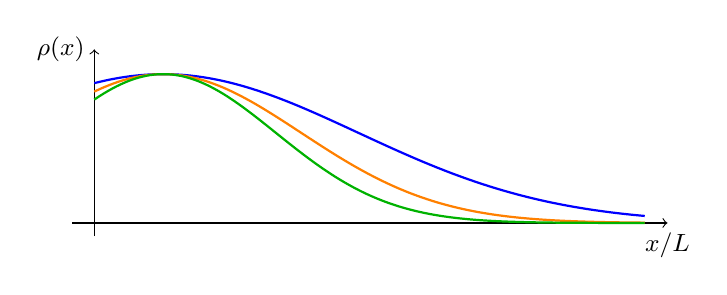
\begin{tikzpicture}[
        x=7cm, y=2.1cm, font=\small,
        declare function={
          rhoBlue(\x)=0.9*exp(-4*(\x-0.125)^2);
          rhoOrange(\x)=0.9*exp(-8*(\x-0.125)^2);
          rhoGreen(\x)=0.9*exp(-12*(\x-0.125)^2);
        }]

  % axes ----------------------------------------------------
  \draw[->] (-0.04,0) -- (1.04,0) node[below] {$x/L$};
  \draw[->] (0,-0.08) -- (0,1.05) node[left] {$\rho(x)$};

  % three density profiles ---------------------------------
  \draw[blue,   thick, smooth, domain=0:1, samples=120]
        plot (\x,{rhoBlue(\x)});
  \draw[orange, thick, smooth, domain=0:1, samples=120]
        plot (\x,{rhoOrange(\x)});
  \draw[green!70!black, thick, smooth, domain=0:1, samples=120]
        plot (\x,{rhoGreen(\x)});

\end{tikzpicture}
}%
  \caption{Entropy density \(\rho(x)\) for three barrier contrasts.
           Colours: blue \(D_{\mathrm{bar}}/D_{\mathrm{in}}=10^{-1}\),
           orange \(10^{-2}\), green \(10^{-3}\).}
  \label{fig:entropy_density}
\end{figure}


\paragraph{Source–sink balance.}
Table \ref{tab:sigma} records the effective source term
\(\sigma=-\partial_t\rho\) averaged over the two pockets at
steady state; values match the informational force prediction
\(\mathbf f=-\rho\nabla D^{-1}\).

\begin{table}[ht]
\centering
\caption{Pocket‐averaged \(\sigma\) for three barrier contrasts
         (Kick units).}
\label{tab:sigma}
\begin{tabular}{ccc}
\toprule
\(D_{\mathrm{bar}}/D_{\mathrm{in}}\) & Left pocket \(\langle\sigma\rangle\) & Right pocket \(\langle\sigma\rangle\) \\
\midrule
$10^{-1}$ & $-3.2\times10^{-4}$ & $+3.2\times10^{-4}$ \\
$10^{-2}$ & $-1.1\times10^{-3}$ & $+1.1\times10^{-3}$ \\
$10^{-3}$ & $-3.5\times10^{-3}$ & $+3.6\times10^{-3}$ \\
\bottomrule
\end{tabular}
\end{table}

\paragraph{Interpretation.}
As the barrier contrast deepens, the informational force
\(|\mathbf f|\propto\nabla D^{-1}\) grows, expelling uncertainty
from the central region and increasing the sink/source magnitude
symmetrically at the pockets—numerical confirmation of the boxed force
law (Sec.~\ref{sec:info_force}).
